Submitted:

\begin{verbatim}[1, 3]\end{verbatim}

Chosen option 1 is available?\begin{quote}Yes.\end{quote}Chosen option 3 is available?\begin{quote}Yes.\end{quote}Remarks on your solution:

All given class diagrams are correct?

\begin{quote}\begin{verbatim}No.\end{verbatim}\end{quote}

The correct solution is:\begin{verbatim}[2,4]\end{verbatim}

Your answer to class diagram 1 is not correct.

Class diagram 1 is invalid.

If for example the inheritance where E inherits from B would not be there, it would be valid.

Your answer to class diagram 2 is not correct.

Class diagram 2 is valid.

The relationships in the class diagram could be named in the following way:



\begin{centering}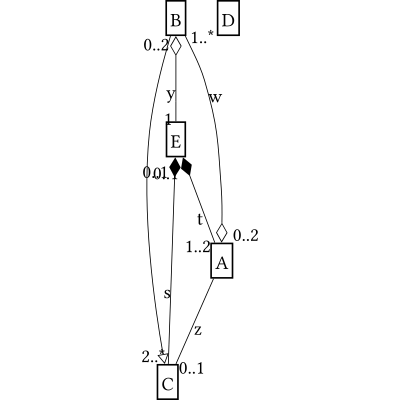
\includegraphics[min width=0.4\textwidth=0.6\textwidth,min height=0.4\textwidth=0.6\textwidth,keepaspectratio,max width=0.9\textwidth,max height=0.9\textwidth]{51/cd32786ed7955f75f2e4050d7464df637cf40075b2d129bb678089584e2eed975201af83b04c596701db35357ce8aed00a3a92e08161.pdf}\end{centering}



Now consider the following object diagram, which is an instance of this class diagram:



\begin{centering}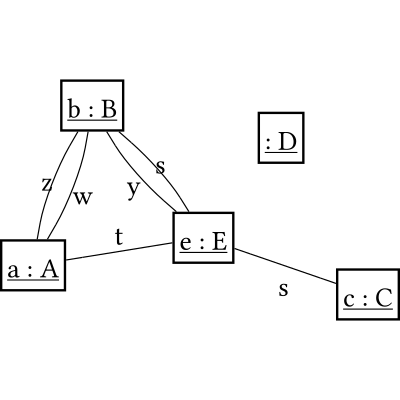
\includegraphics[min width=0.4\textwidth=0.6\textwidth,min height=0.4\textwidth=0.6\textwidth,keepaspectratio,max width=0.9\textwidth,max height=0.9\textwidth]{51/odcc69f5b1d023e969782ea5f974f3b12438efcf1e7d340bc3f501216ae3567bdf13.pdf}\end{centering}



Your answer to class diagram 3 is not correct.

Class diagram 3 is invalid.

If for example the inheritance where E inherits from B would not be there, it would be valid.

Your answer to class diagram 4 is not correct.

Class diagram 4 is valid.

The relationships in the class diagram could be named in the following way:



\begin{centering}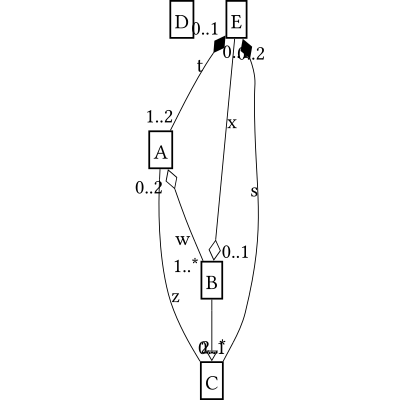
\includegraphics[min width=0.4\textwidth=0.6\textwidth,min height=0.4\textwidth=0.6\textwidth,keepaspectratio,max width=0.9\textwidth,max height=0.9\textwidth]{51/cd3faf14323c0cc9a0be4d24da2f2bee302bf2951cb8edca73b19f0e1599317b0301af83b04c596701db35357ce8aed00a3a92e08161.pdf}\end{centering}



Now consider the following object diagram, which is an instance of this class diagram:



\begin{centering}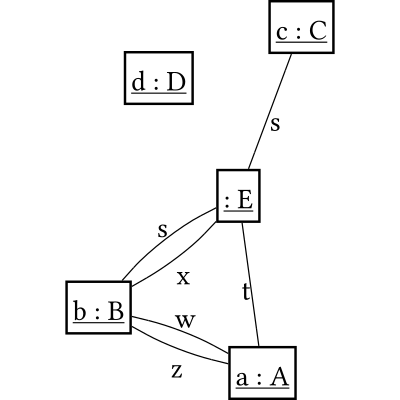
\includegraphics[min width=0.4\textwidth=0.6\textwidth,min height=0.4\textwidth=0.6\textwidth,keepaspectratio,max width=0.9\textwidth,max height=0.9\textwidth]{51/odbad91f15a5a868e5e1adda232caffabf7a2c51c009dd1f35b88c91083fb9330013.pdf}\end{centering}



